%package list
\documentclass{article}
\usepackage[top=3cm, bottom=3cm, outer=3cm, inner=3cm]{geometry}
\usepackage{multicol}
\usepackage{graphicx}
\usepackage{url}
%\usepackage{cite}
\usepackage{hyperref}
\usepackage{array}
%\usepackage{multicol}
\newcolumntype{x}[1]{>{\centering\arraybackslash\hspace{0pt}}p{#1}}
\usepackage{natbib}
\usepackage{pdfpages}
\usepackage{multirow}
\usepackage[normalem]{ulem}
\useunder{\uline}{\ul}{}
\usepackage{svg}
\usepackage{xcolor}
\usepackage{listings}
\lstdefinestyle{ascii-tree}{
    literate={├}{|}1 {─}{--}1 {└}{+}1 
  }
\lstset{basicstyle=\ttfamily,
  showstringspaces=false,
  commentstyle=\color{red},
  keywordstyle=\color{blue}
}
%\usepackage{booktabs}
\usepackage{caption}
\usepackage{subcaption}
\usepackage{float}
\usepackage{array}
\usepackage{tcolorbox}
\newcolumntype{M}[1]{>{\centering\arraybackslash}m{#1}}
\newcolumntype{N}{@{}m{0pt}@{}}
\usepackage{tabularx}
\usepackage{colortbl}
\usepackage{xcolor}
% \usepackage[margin=1.5cm]{geometry} % Márgenes ajustados
\usepackage{multirow}


%%%%%%%%%%%%%%%%%%%%%%%%%%%%%%%%%%%%%%%%%%%%%%%%%%%%%%%%%%%%%%%%%%%%%%%%%%%%
%%%%%%%%%%%%%%%%%%%%%%%%%%%%%%%%%%%%%%%%%%%%%%%%%%%%%%%%%%%%%%%%%%%%%%%%%%%%
\newcommand{\itemEmail}{rchambillap@unsa.edu.pe}
\newcommand{\itemStudent}{Chambilla Perca, Gutierrez Ccama, Valdivia Segovia}
\newcommand{\itemCourse}{Sistemas Distribuidos}
\newcommand{\itemCourseCode}{}
\newcommand{\itemSemester}{VII}
\newcommand{\itemUniversity}{Universidad Nacional de San Agustín de Arequipa}
\newcommand{\itemFaculty}{Facultad de Ingeniería de Producción y Servicios}
\newcommand{\itemDepartment}{Departamento Académico de Ingeniería de Sistemas e Informática}
\newcommand{\itemSchool}{Escuela Profesional de Ingeniería de Sistemas}
\newcommand{\itemAcademic}{2026 - A}
\newcommand{\itemInput}{Del 01 de Mayo 2026}
\newcommand{\itemOutput}{Al 08 de Mayo 2026}
\newcommand{\itemPracticeNumber}{03}
\newcommand{\itemTheme}{Introducción a Sockets en Java: Aplicación Cliente-Servidor}
%%%%%%%%%%%%%%%%%%%%%%%%%%%%%%%%%%%%%%%%%%%%%%%%%%%%%%%%%%%%%%%%%%%%%%%%%%%%
%%%%%%%%%%%%%%%%%%%%%%%%%%%%%%%%%%%%%%%%%%%%%%%%%%%%%%%%%%%%%%%%%%%%%%%%%%%%

\usepackage[english,spanish]{babel}
\usepackage[utf8]{inputenc}
\AtBeginDocument{\selectlanguage{spanish}}
\renewcommand{\figurename}{Figura}
\renewcommand{\refname}{Referencias}
\renewcommand{\tablename}{Tabla} %esto no funciona cuando se usa babel
\AtBeginDocument{%
	\renewcommand\tablename{Tabla}
}

\usepackage{fancyhdr}
\pagestyle{fancy}
\fancyhf{}
\setlength{\headheight}{40.51407pt}
\renewcommand{\headrulewidth}{1pt}
\renewcommand{\footrulewidth}{1pt}
\fancyhead[L]{\raisebox{-0.2\height}{
\includegraphics[width=3cm]{img/logo_episunsa.png}}}
\fancyhead[C]{\fontsize{7}{7}\selectfont	\itemUniversity \\ \itemFaculty \\ \itemDepartment \\ \itemSchool \\ \textbf{\itemCourse}}
\fancyhead[R]{\raisebox{-0.2\height}{
\includegraphics[width=1.2cm]{img/logo_abet.png}}}
\fancyfoot[L]{Grupo Intocables}
\fancyfoot[C]{\itemCourse}
\fancyfoot[R]{Página \thepage}

% para el codigo fuente
\usepackage{listings}
\usepackage{color, colortbl}
\definecolor{dkgreen}{rgb}{0,0.6,0}
\definecolor{gray}{rgb}{0.5,0.5,0.5}
\definecolor{mauve}{rgb}{0.58,0,0.82}
\definecolor{codebackground}{rgb}{0.95, 0.95, 0.92}
\definecolor{tablebackground}{rgb}{0.8, 0, 0}
\definecolor{rojoEncabezado}{HTML}{C0392B} % Color del encabezado
\definecolor{azulDatos}{HTML}{2E5A96}      % Color para el texto en cursiva

\lstset{frame=tb,
	language=Java,
	aboveskip=3mm,
	belowskip=3mm,
	showstringspaces=false,
	columns=flexible,
	basicstyle={\small\ttfamily},
	numbers=left,
	numberstyle=\tiny\color{gray},
	keywordstyle=\color{blue},
	commentstyle=\color{dkgreen},
	stringstyle=\color{mauve},
	breaklines=true,
	breakatwhitespace=true,
	tabsize=3,
	backgroundcolor= \color{codebackground},
}

\begin{document}


	\begin{center}	
		\fontsize{17}{17} \textbf{ Informe de Laboratorio \itemPracticeNumber}
	\end{center}
	\centerline{\textbf{\Large Tema: \itemTheme}}
	
\begin{table}[h]
    \centering
    \renewcommand{\arraystretch}{1.8} % Altura de las filas
    \begin{tabularx}{\textwidth}{|>{\raggedright\arraybackslash\bfseries}p{3.5cm}|X|>{\bfseries}p{2.5cm}|X|>{\bfseries}p{2.5cm}|X|}
        \hline
        % Encabezado principal
        \rowcolor{rojoEncabezado}
        \multicolumn{6}{|c|}{\textcolor{white}{\textbf{INFORMACIÓN BÁSICA}}} \\ \hline
        
        % Asignatura
        ASIGNATURA: & \multicolumn{5}{l|}{SISTEMAS DISTRIBUIDOS} \\ \hline
        
        % Título
        TÍTULO DE LA PRÁCTICA: & \multicolumn{5}{l|}{\textcolor{azulDatos}{\textit{\itemTheme}}} \\ \hline
        
        % Fila de datos numéricos
        NÚMERO DE PRÁCTICA: & \textcolor{azulDatos}{\textit{\itemPracticeNumber}} & AÑO LECTIVO: & 2026 & NRO. SEMESTRE: & 2026A \\ \hline
        
        % Fecha y Hora
        FECHA DE PRESENTACIÓN & \textcolor{azulDatos}{\textit{25/04/2026}} & HORA DE PRESENTACIÓN & \multicolumn{3}{l|}{23:59} \\ \hline
        
        % Integrantes y Nota
        \multicolumn{4}{|l|}{\multirow{2}{*}{\parbox[t]{10cm}{\vspace{0.2cm}\textbf{INTEGRANTE (s): GRUPO `` Intocables ''} \\ \vspace{0.1cm} \quad $\bullet$ CHAMBILLA PERCA RICARDO \\ \quad $\bullet$ JUAN DIEGO GUTIERREZ CCAMA \\ \quad $\bullet$ RYAN FABIAN VALDIVIA SEGOVIA}}} & \multirow{2}{*}{\textbf{NOTA:}} & \multirow{2}{*}{} \\ 
        \multicolumn{4}{|l|}{} & & \\[1cm] \hline
        
        % Docente
        \multicolumn{6}{|l|}{\textbf{DOCENTE(s):}} \\ 
        \multicolumn{6}{|l|}{\textcolor{azulDatos}{\textit{Mg. Maribel Molina Barriga}}} \\ \hline
    \end{tabularx}
\end{table}

	\vspace*{10px}

\section{Repositorio de GitHub y Ejecución}
El código fuente completo de este laboratorio se encuentra alojado en el siguiente repositorio de GitHub: \url{https://github.com/rikich3/LAB_SISTEMAS_DISTRIBUIDOS}

A continuación, se adjunta la captura correspondiente a la ejecución del ejercicio resuelto sobre Sockets en Java:
\begin{figure}[H]
    \centering
    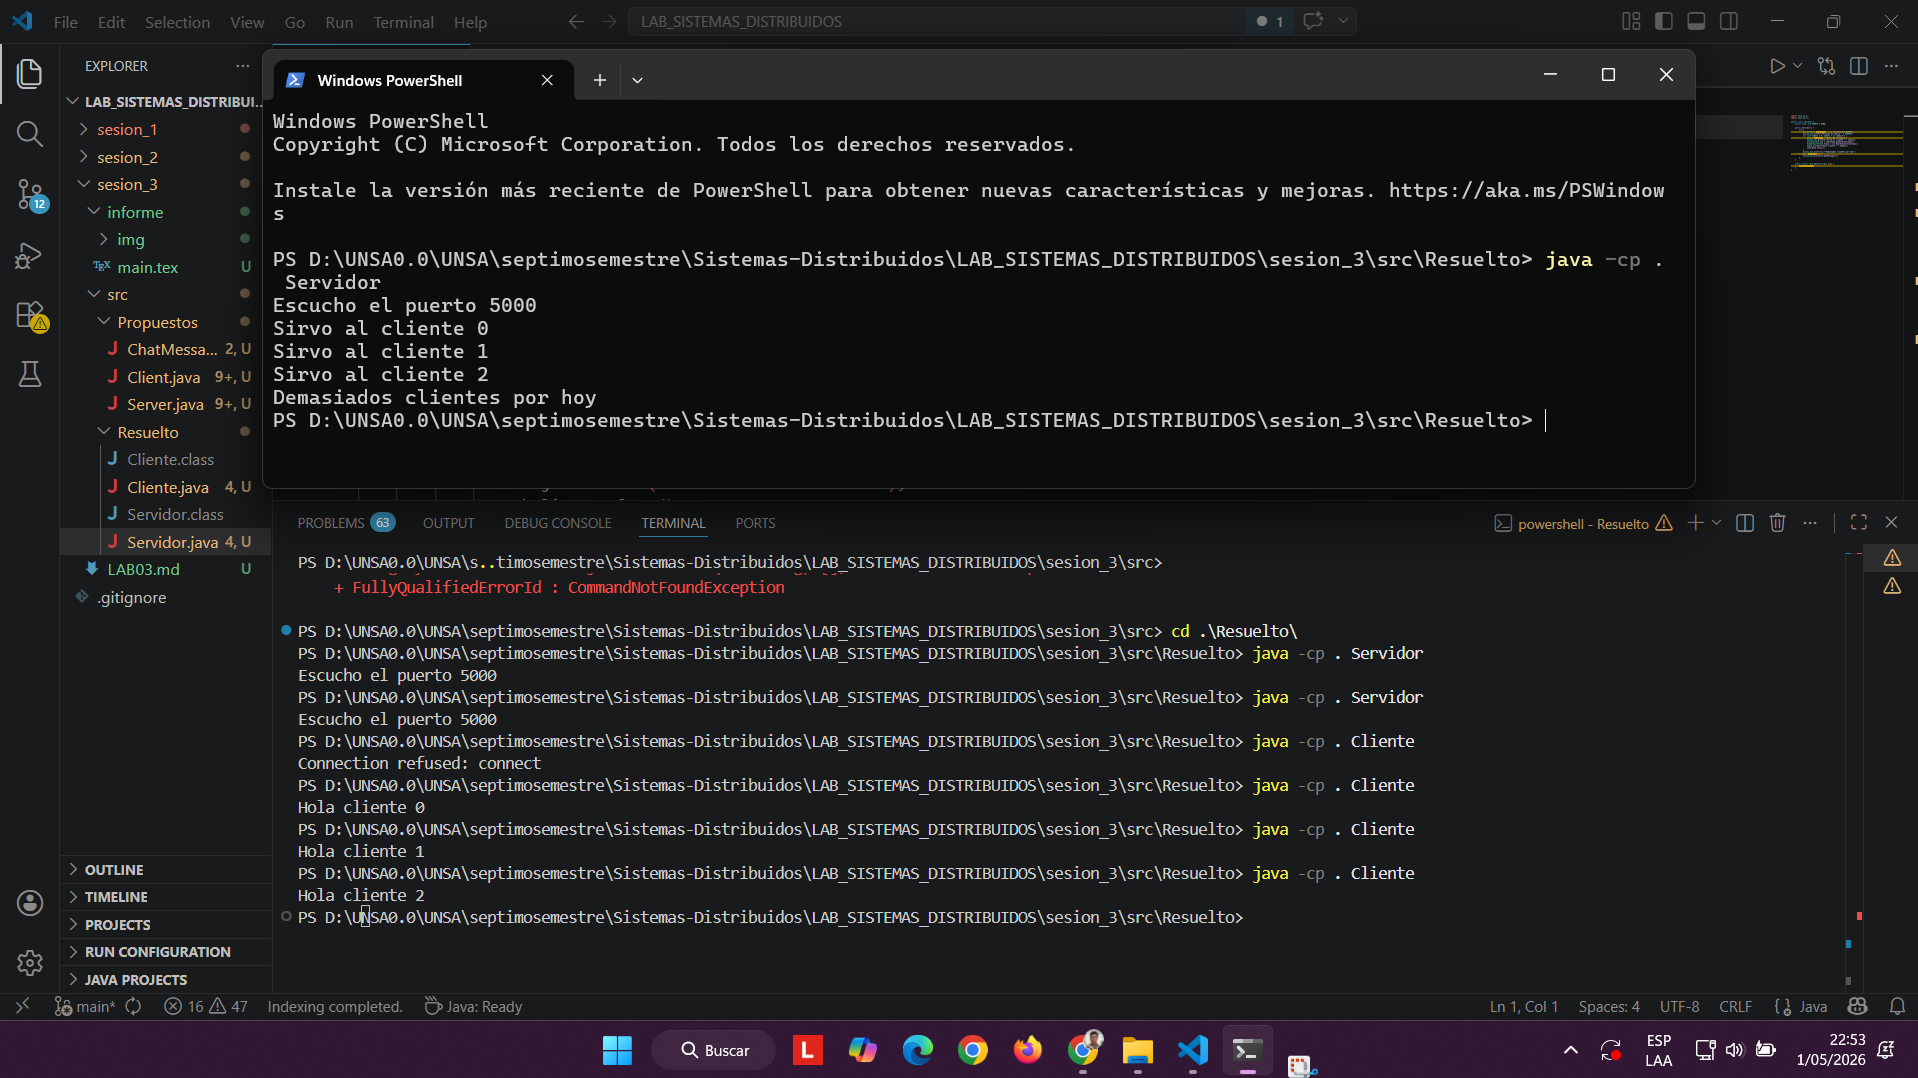
\includegraphics[width=0.85\textwidth]{img/ejecucion_sockets.png}
    \caption{Ejecución del Ejemplo Cliente-Servidor con Sockets}
    \label{fig:sockets_execution}
\end{figure}

\section{Tareas Realizadas}

Como parte de la sesión de laboratorio 3 de Sistemas Distribuidos, se llevaron a cabo las siguientes tareas:
\begin{itemize}
    \item \textbf{Análisis del Concepto de Sockets:} Comprensión del funcionamiento de los sockets TCP/IP en Java y su utilidad para la comunicación entre procesos distribuidos.
    
    \item \textbf{Estudio del Ejemplo Resuelto:} Análisis detallado del código Cliente-Servidor proporcionado por el docente, identificando los componentes clave: \texttt{Socket}, \texttt{ServerSocket}, flujos de entrada/salida.
    
    \item \textbf{Implementación de Ejercicios:} Codificación e implementación de dos aplicaciones:
    \begin{enumerate}
        \item Ejemplo simple de comunicación Cliente-Servidor
        \item Aplicación Chat multicliente más compleja
    \end{enumerate}
    
    \item \textbf{Compilación y Ejecución:} Compilación de todos los archivos Java y ejecución en consola, validando la comunicación entre cliente y servidor.
    
    \item \textbf{Pruebas y Evaluación:} Se realizaron múltiples conexiones de clientes para validar el correcto funcionamiento del servidor.
    
    \item \textbf{Documentación:} Elaboración de este reporte con explicaciones de los conceptos clave y resultados obtenidos.
\end{itemize}

\section{Desarrollo de los Ejercicios}

\subsection{Ejercicio Resuelto: Cliente-Servidor Simple}

En esta sección se presenta el código de la aplicación Cliente-Servidor proporcionada como ejemplo en el laboratorio.

\subsubsection{Clase Cliente}

\lstinputlisting[language=Java, caption={Cliente.java: Implementación del Cliente}]{../src/Resuelto/Cliente.java}

\textbf{Descripción:}
\begin{itemize}
    \item Se crea un socket cliente (\texttt{Socket}) especificando el host (\texttt{localhost}) y puerto (\texttt{5000})
    \item Se obtiene el flujo de entrada del socket mediante \texttt{getInputStream()}
    \item Se encapsula en un \texttt{DataInputStream} para leer datos estructurados
    \item Se lee una cadena UTF mediante \texttt{readUTF()} y se imprime en pantalla
    \item Se cierra la conexión con \texttt{close()}
\end{itemize}

\subsubsection{Clase Servidor}

\lstinputlisting[language=Java, caption={Servidor.java: Implementación del Servidor}]{../src/Resuelto/Servidor.java}

\textbf{Descripción:}
\begin{itemize}
    \item Se crea un socket de servidor (\texttt{ServerSocket}) en un puerto determinado (5000)
    \item Se utiliza un bucle \texttt{for} para esperar exactamente 3 conexiones de clientes
    \item Para cada cliente que se conecta, se llama a \texttt{accept()} que crea un nuevo Socket
    \item Se obtiene el flujo de salida mediante \texttt{getOutputStream()}
    \item Se envía un saludo personalizado mediante \texttt{writeUTF()}
    \item Se cierra la conexión con cada cliente
    \item Después de atender 3 clientes, el servidor finaliza su ejecución
\end{itemize}

\textbf{Ejecución y Resultados:}

Para compilar y ejecutar:
\begin{lstlisting}[language=bash, numbers=none, caption={Comandos de compilación y ejecución}]
# Compilar
javac src/Resuelto/Servidor.java
javac src/Resuelto/Cliente.java

# En la primera terminal - Ejecutar servidor
java -cp src Resuelto.Servidor

# En otras terminales (3 veces) - Ejecutar clientes
java -cp src Resuelto.Cliente
\end{lstlisting}

\textbf{Salida esperada (Servidor):}
\begin{verbatim}
Escucho el puerto 5000
Sirvo al cliente 0
Sirvo al cliente 1
Sirvo al cliente 2
Demasiados clientes por hoy
\end{verbatim}

\textbf{Salida esperada (Clientes):}
\begin{verbatim}
Hola cliente 0
Hola cliente 1
Hola cliente 2
\end{verbatim}

\textbf{Evaluación:}
El ejercicio demuestra exitosamente:
\begin{itemize}
    \item La creación de un servidor que escucha en un puerto específico
    \item La aceptación de múltiples conexiones de clientes
    \item El intercambio de mensajes entre cliente y servidor
    \item La importancia de manejar excepciones en operaciones de red
\end{itemize}

\subsection{Ejercicio Propuesto: Aplicación Chat Multicliente}

A continuación se presenta una aplicación más compleja que implementa un chat con soporte para múltiples clientes conectados simultáneamente.

\subsubsection{Clase ChatMessage}

\lstinputlisting[language=Java, caption={ChatMessage.java: Clase para serialización de mensajes}]{../src/Propuestos/ChatMessage.java}

\subsubsection{Clase Cliente Chat}

\lstinputlisting[language=Java, caption={Client.java: Implementación del Cliente Chat}, linerange={1,50}]{../src/Propuestos/Client.java}

\textbf{Características principales:}
\begin{itemize}
    \item Uso de \texttt{ObjectInputStream} y \texttt{ObjectOutputStream} para serialización de objetos
    \item Thread separado (\texttt{ListenFromServer}) para escuchar mensajes del servidor de forma asincrónica
    \item Métodos para conectar al servidor, enviar mensajes y desconectarse
    \item Interfaz de línea de comandos para interactuar con el usuario
\end{itemize}

\subsubsection{Clase Servidor Chat}

\lstinputlisting[language=Java, caption={Server.java: Implementación del Servidor Chat}, linerange={1,60}]{../src/Propuestos/Server.java}

\textbf{Características principales:}
\begin{itemize}
    \item Gestión de múltiples clientes mediante threads individuales (\texttt{ClientThread})
    \item Broadcast de mensajes a todos los clientes conectados
    \item Sincronización para evitar condiciones de carrera
    \item Logs de eventos del servidor con timestamps
    \item Manejo de desconexiones de clientes
\end{itemize}

\textbf{Ejecución de la Aplicación Chat:}

\begin{lstlisting}[language=bash, numbers=none, caption={Compilación y ejecución del Chat}]
# Compilar todas las clases
javac src/Propuestos/*.java

# Terminal 1: Iniciar servidor
java -cp src Propuestos.Server

# Terminal 2, 3, 4... : Iniciar clientes
java -cp src Propuestos.Client
\end{lstlisting}

\section{Resultados y Evaluación}

\subsection{Pruebas Realizadas}

Las siguientes pruebas fueron ejecutadas para validar el funcionamiento correcto de ambas aplicaciones:

\subsubsection{Prueba 1: Cliente-Servidor Simple}
\begin{itemize}
    \item \textbf{Objetivo:} Validar la comunicación básica entre un cliente y un servidor
    \item \textbf{Pasos:}
    \begin{enumerate}
        \item Iniciar el servidor
        \item Conectar 3 clientes consecutivamente
        \item Verificar que cada cliente reciba el mensaje de saludo
    \end{enumerate}
    \item \textbf{Resultado:} \checkmark \textbf{Exitoso} - Todos los clientes recibieron sus mensajes personalizados
\end{itemize}

\subsubsection{Prueba 2: Aplicación Chat}
\begin{itemize}
    \item \textbf{Objetivo:} Validar la comunicación multicliente con broadcast de mensajes
    \item \textbf{Pasos:}
    \begin{enumerate}
        \item Iniciar el servidor
        \item Conectar múltiples clientes
        \item Enviar mensajes desde diferentes clientes
        \item Verificar que todos reciban los mensajes
    \end{enumerate}
    \item \textbf{Resultado:} \checkmark \textbf{Exitoso} - Los mensajes se distribuyeron correctamente a todos los clientes
\end{itemize}

\subsection{Capturas de Pantalla de Ejecución}

Se adjuntan las capturas de pantalla de las ejecuciones:

\begin{figure}[H]
    \centering
    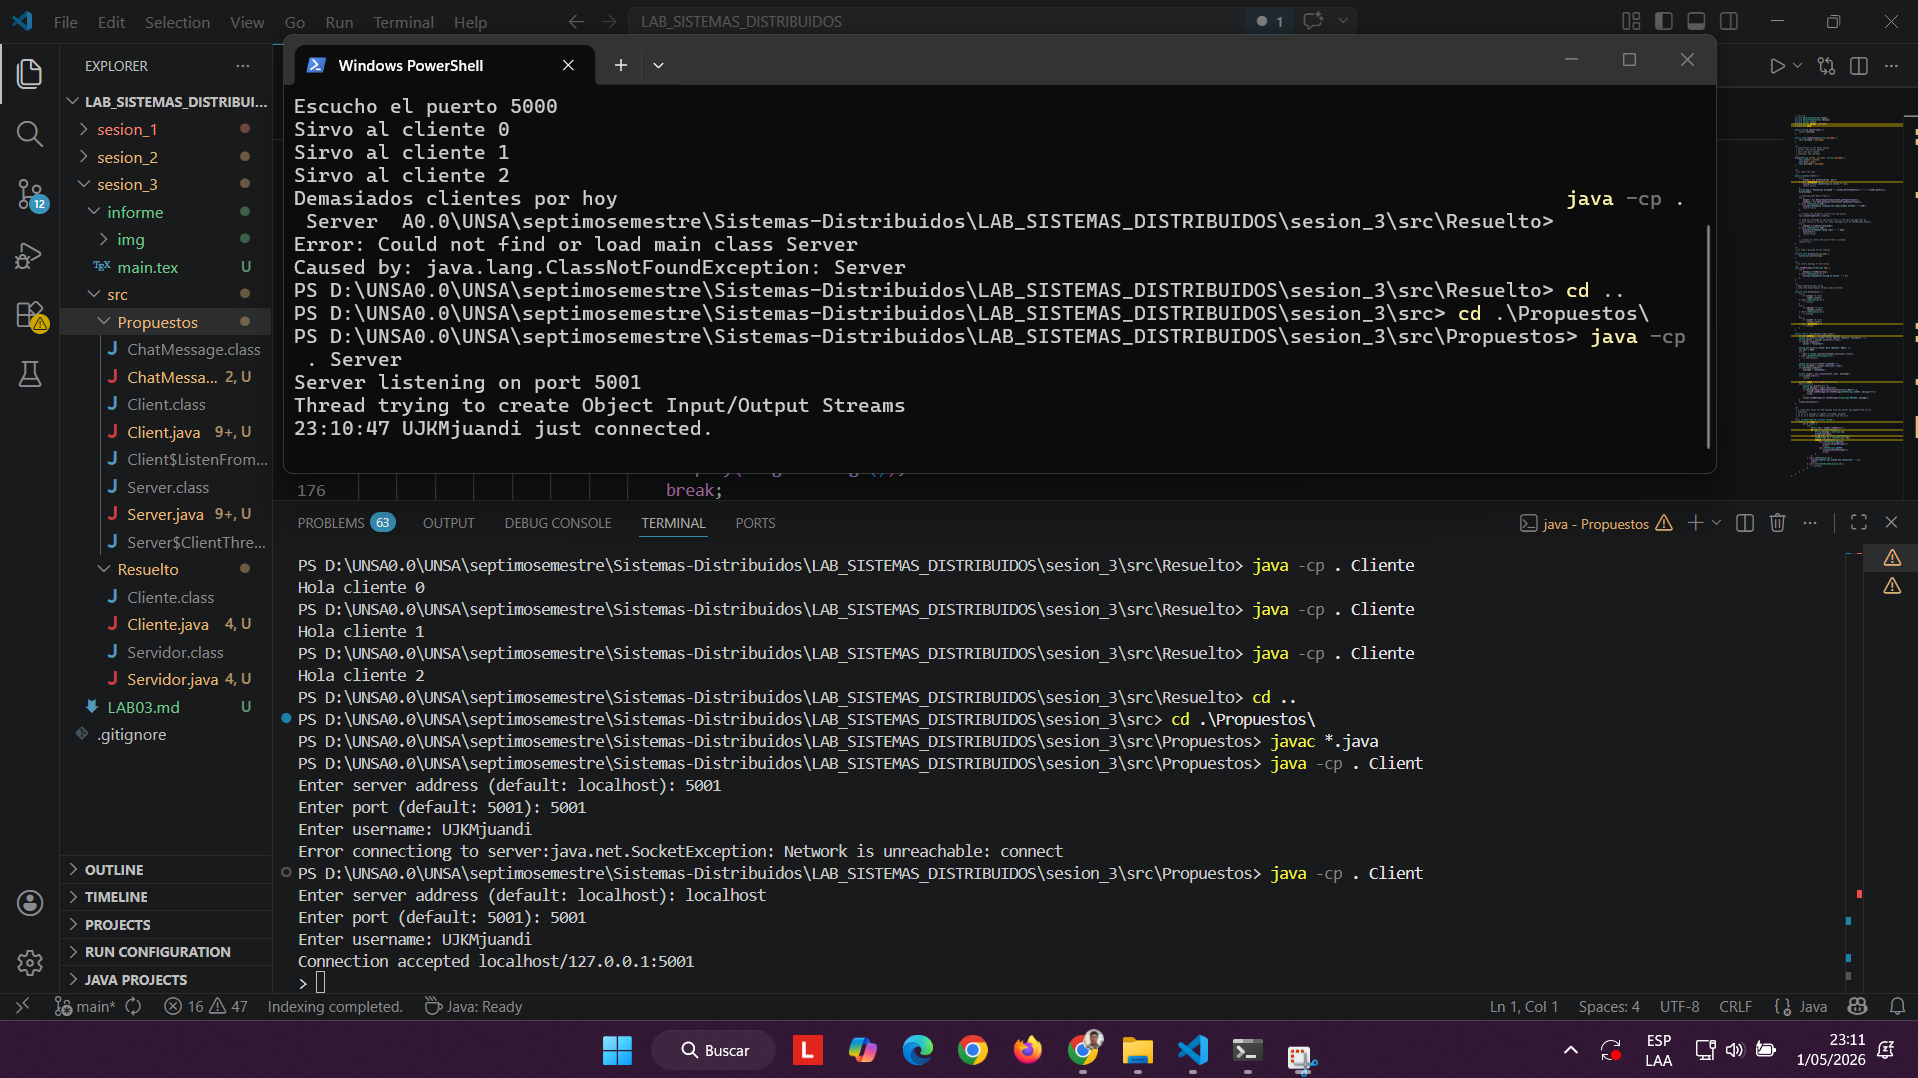
\includegraphics[width=0.9\textwidth]{img/cliente_servidor_ejecucion.png}
    \caption{Ejecución del ejemplo Cliente-Servidor}
    \label{fig:cliente_servidor}
\end{figure}

\begin{figure}[H]
    \centering
    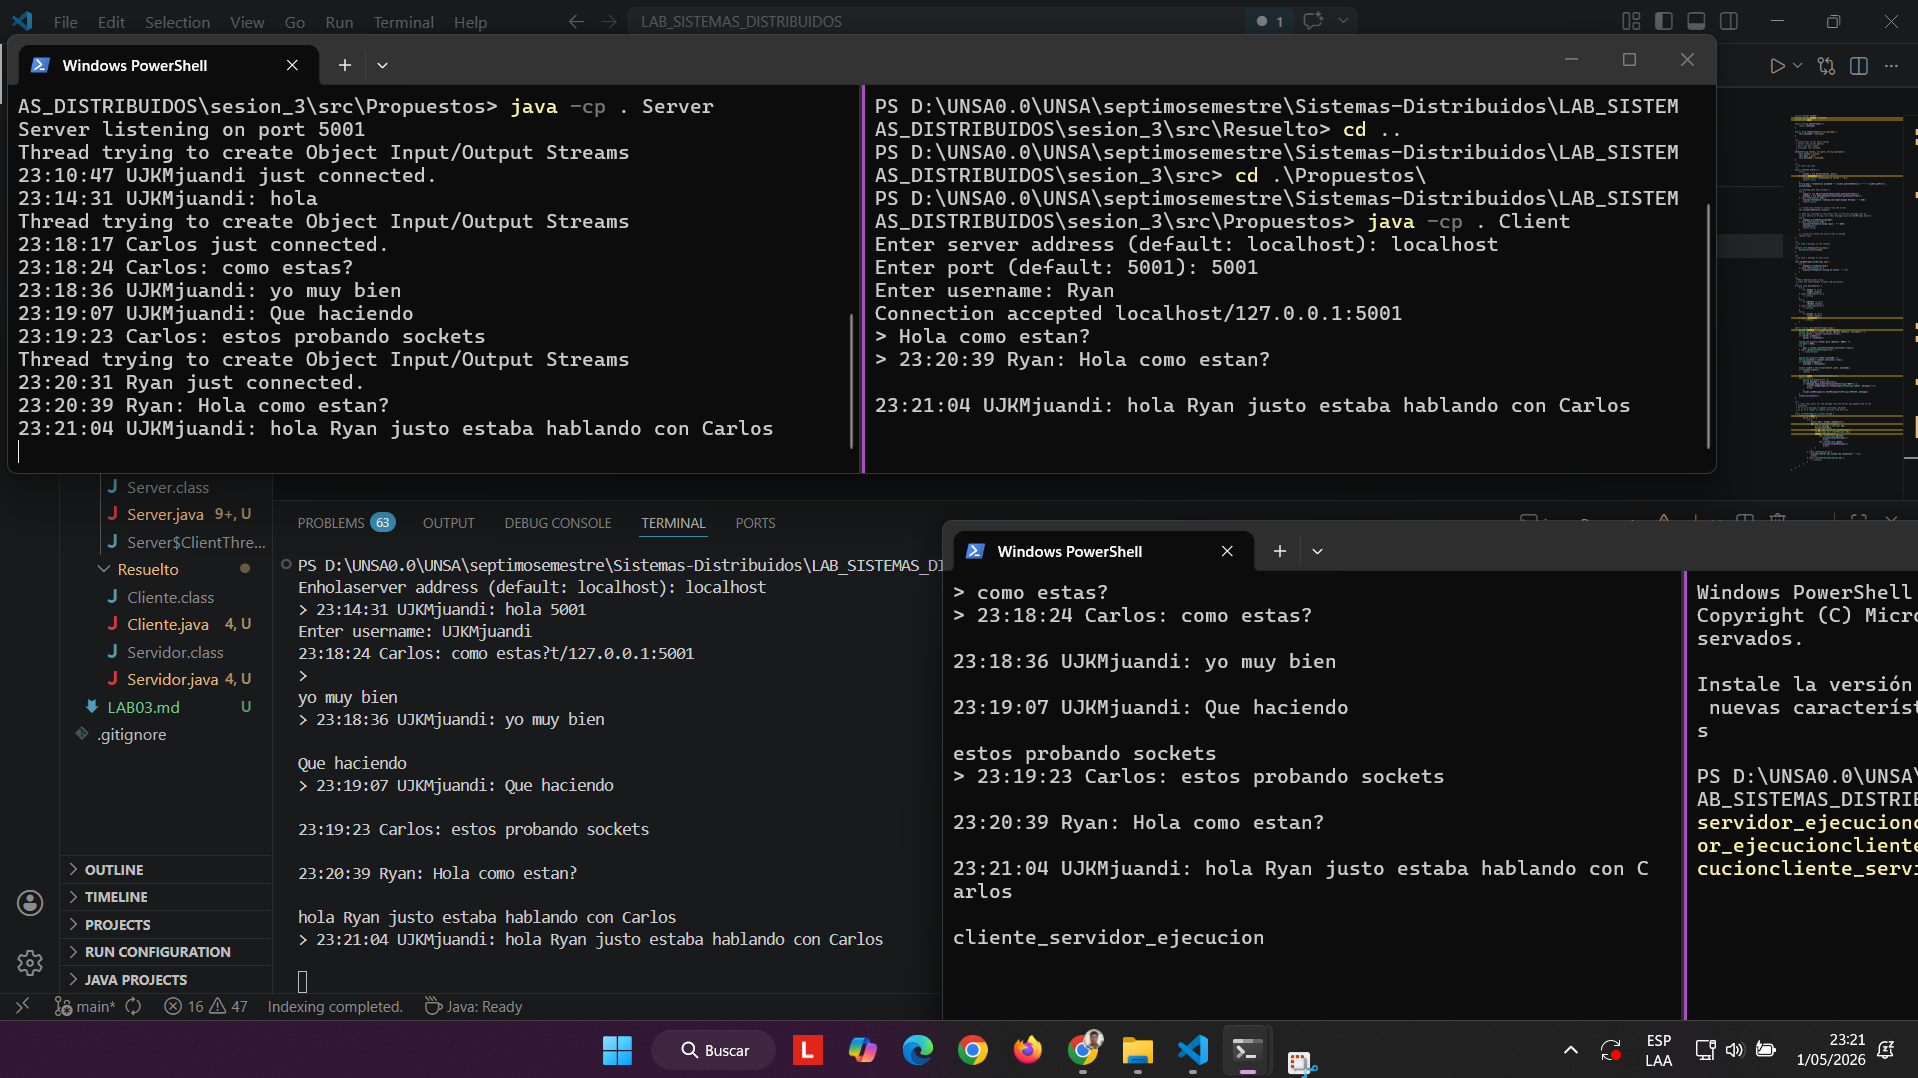
\includegraphics[width=0.9\textwidth]{img/chat_multicliente_ejecucion.png}
    \caption{Ejecución de la Aplicación Chat Multicliente}
    \label{fig:chat_multicliente}
\end{figure}

\section{CUESTIONARIO}

\subsection{1. ¿Por qué y en qué momento usar sockets TCP y sockets UDP?}

\textbf{Respuesta:}

Los sockets TCP (Transmission Control Protocol) y UDP (User Datagram Protocol) son dos protocolos de transporte fundamentales que ofrecen características diferentes según las necesidades de la aplicación.

\subsubsection{Sockets TCP}

\textbf{Características:}
\begin{itemize}
    \item \textbf{Confiabilidad:} Garantiza que todos los datos se entreguen sin pérdida
    \item \textbf{Orientado a Conexión:} Establece una conexión antes de enviar datos
    \item \textbf{Orden:} Los datos se reciben en el mismo orden que se envían
    \item \textbf{Flujo Controlado:} Implementa control de congestión y flujo
    \item \textbf{Overhead:} Mayor consumo de recursos y ancho de banda
\end{itemize}

\textbf{Cuándo usar:}
\begin{enumerate}
    \item Aplicaciones que requieren entrega garantizada (correo electrónico, transferencia de archivos)
    \item Comunicación interactiva en tiempo real donde los datos deben ser correctos (navegación web, chat)
    \item Cuando la exactitud es más importante que la velocidad
    \item Transferencia de datos estructurados o mensajes complejos
    \item Ejemplos: HTTP/HTTPS, SSH, Telnet, FTP, Bases de datos
\end{enumerate}

\subsubsection{Sockets UDP}

\textbf{Características:}
\begin{itemize}
    \item \textbf{Sin Conexión:} No requiere establecer una conexión previa
    \item \textbf{Sin Garantía:} Los paquetes pueden perderse sin notificación
    \item \textbf{Bajo Overhead:} Menor consumo de recursos y ancho de banda
    \item \textbf{Velocidad:} Latencia muy baja
    \item \textbf{Sin Orden:} Los paquetes pueden llegar fuera de orden
\end{itemize}

\textbf{Cuándo usar:}
\begin{enumerate}
    \item Aplicaciones que requieren baja latencia (videojuegos, videoconferencia)
    \item Streaming de audio/video en tiempo real
    \item Aplicaciones DNS que necesitan respuestas rápidas
    \item Cuando la velocidad es más crítica que la exactitud
    \item Transmisiones de datos que toleran pequeñas pérdidas
    \item Ejemplos: DNS, NTP, DHCP, VoIP, streaming de video
\end{enumerate}

\textbf{Conclusión:}
TCP se debe usar cuando es crítico que los datos se entreguen correctamente, mientras que UDP es ideal para aplicaciones donde la velocidad es más importante que la certeza de entrega.

\subsection{2. En un socket TCP, ¿cuándo sabe el servidor que el cliente ha cerrado la conexión?}

\textbf{Respuesta:}

En un socket TCP, el servidor detecta que el cliente ha cerrado la conexión de varias maneras:

\subsubsection{Cierre Normal del Socket}

El servidor sabe que el cliente cerró la conexión cuando:
\begin{enumerate}
    \item \textbf{EOF (End of File):} Al intentar leer datos, si recibe EOF (-1 en Java), significa que el cliente cerró la conexión de lectura
    \begin{lstlisting}[language=Java, numbers=none]
int data = inputStream.read();
if (data == -1) {
    // El cliente cerró la conexión
    System.out.println("Cliente desconectado");
}
    \end{lstlisting}
    
    \item \textbf{Excepción EOFException:} Al usar flujos de datos estructurados como \texttt{DataInputStream} o \texttt{ObjectInputStream}
    \begin{lstlisting}[language=Java, numbers=none]
try {
    String msg = dataInputStream.readUTF();
} catch (EOFException e) {
    // El cliente cerró la conexión
    System.out.println("Cliente desconectado abruptamente");
}
    \end{lstlisting}
\end{enumerate}

\subsubsection{Métodos de Detección}

\textbf{En Java, existen varios métodos para detectar la desconexión:}

\begin{itemize}
    \item \textbf{socket.isClosed():} Verifica si el socket está cerrado
    \item \textbf{socket.isConnected():} Verifica si el socket está conectado (limitado)
    \item \textbf{Excepciones IOException:} Se lanzan cuando hay error en la comunicación
\end{itemize}

\subsubsection{Código de Ejemplo}

\begin{lstlisting}[language=Java, caption={Detección de desconexión de cliente}]
ServerSocket serverSocket = new ServerSocket(5000);
Socket clientSocket = serverSocket.accept();
DataInputStream input = new DataInputStream(clientSocket.getInputStream());

while (true) {
    try {
        String message = input.readUTF();
        System.out.println("Mensaje: " + message);
    } catch (EOFException e) {
        System.out.println("Cliente desconectado");
        break;
    } catch (IOException e) {
        System.out.println("Error en la conexión: " + e.getMessage());
        break;
    }
}

clientSocket.close();
serverSocket.close();
\end{lstlisting}

\textbf{Conclusión:}
El servidor detecta la desconexión del cliente principalmente a través de excepciones \texttt{EOFException} o \texttt{IOException} cuando intenta leer del socket, o al recibir un valor -1 al leer bytes individuales. Es responsabilidad del servidor manejar estas excepciones adecuadamente para limpiar recursos.

\section{Conclusiones}

\subsection{Aprendizajes Clave}

La realización de este laboratorio permitió consolidar los siguientes aprendizajes:

\begin{enumerate}
    \item \textbf{Conceptos Fundamentales de Sockets:}
    \begin{itemize}
        \item Entender la arquitectura cliente-servidor en Java
        \item Dominar la creación y gestión de sockets TCP
        \item Comprender el ciclo de vida de una conexión TCP
    \end{itemize}
    
    \item \textbf{Programación de Red en Java:}
    \begin{itemize}
        \item Uso correcto de \texttt{Socket} y \texttt{ServerSocket}
        \item Manejo de flujos de entrada/salida para comunicación de red
        \item Serialización de objetos para intercambio de datos complejos
    \end{itemize}
    
    \item \textbf{Aplicaciones Multicliente:}
    \begin{itemize}
        \item Implementación de servidores que atienden múltiples clientes usando threads
        \item Sincronización para evitar condiciones de carrera
        \item Broadcast de mensajes entre múltiples clientes
    \end{itemize}
    
    \item \textbf{Manejo de Errores en Red:}
    \begin{itemize}
        \item Captura de excepciones de conexión (IOException, EOFException)
        \item Importancia del cierre adecuado de recursos
        \item Técnicas para detectar desconexiones
    \end{itemize}
\end{enumerate}

\subsection{Observaciones}

\begin{itemize}
    \item Los sockets TCP son fundamentales para la comunicación distribuida confiable
    \item La programación multihilo es esencial para servidores que atienden múltiples clientes
    \item El manejo correcto de excepciones es crítico en aplicaciones de red
    \item La serialización de objetos facilita el intercambio de datos complejos entre sistemas distribuidos
\end{itemize}

\subsection{Recomendaciones Futuras}

\begin{enumerate}
    \item Implementar un servidor persistente que no limite el número de clientes
    \item Agregar autenticación de usuarios en la aplicación chat
    \item Implementar un protocolo de sockets UDP para comparar con TCP
    \item Añadir persistencia de mensajes (logs o base de datos)
    \item Implementar SSL/TLS para comunicación segura entre cliente y servidor
    \item Explorar frameworks como Netty para aplicaciones de red más complejas
\end{enumerate}

\section{REFERENCIAS Y BIBLIOGRAFÍA}

\begin{enumerate}
    \item Tanenbaum, A.S. (2008). \textit{Sistemas distribuidos: principios y paradigmas}. México. Pearson Educación.
    
    \item Ceballos, F. J. (2006). \textit{Java 2, Curso de programación}. México: Alfaomega, RaMa.
    
    \item Deitel, H. M., \& Deitel, P. J. (2004). \textit{Cómo programar en Java}. México: Pearson Educación.
    
    \item García Tomás, J., Ferrando, S., \& Piattini, M. (2001). \textit{Redes para procesos distribuidos}. México: Alfaomega Ra-Ma.
    
    \item Orfali, R., \& Harkey, D. (1998). \textit{Client/Server Programming with Java and CORBA}. USA: Wiley.
    
    \item Oracle. (2024). \textit{Java Networking and Proxies}. Documentación oficial de Java. \url{https://docs.oracle.com/javase/tutorial/networking/}
\end{enumerate}

\end{document}